\section{Model implementation}\label{sec:implementation}

The main module of our implementation is the \code{User} module, so we will
start discussing it first.

\figref{fig:userfsm} shows the finite-state machine (FSM) diagram of the
\code{User} module. Exchanged messages are represented in upper case. Additional
conditions to move from one state to another are shown inside square brackets.
Operations on counter variables (\code{counter} and \code{slotcount}) are shown
in \textit{italic}. Symbols \(m\), \(T\) and \(\delta\) represents,
respectively, the parameters \code{maxCopies}, \code{hearWindow} and
\code{relayDelay}. Note that the \code{RELAYING} state is not really a state,
since it is instantaneous: it represents the action of relaying the message
before stopping.

\begin{figure}[htb]
	\centering
	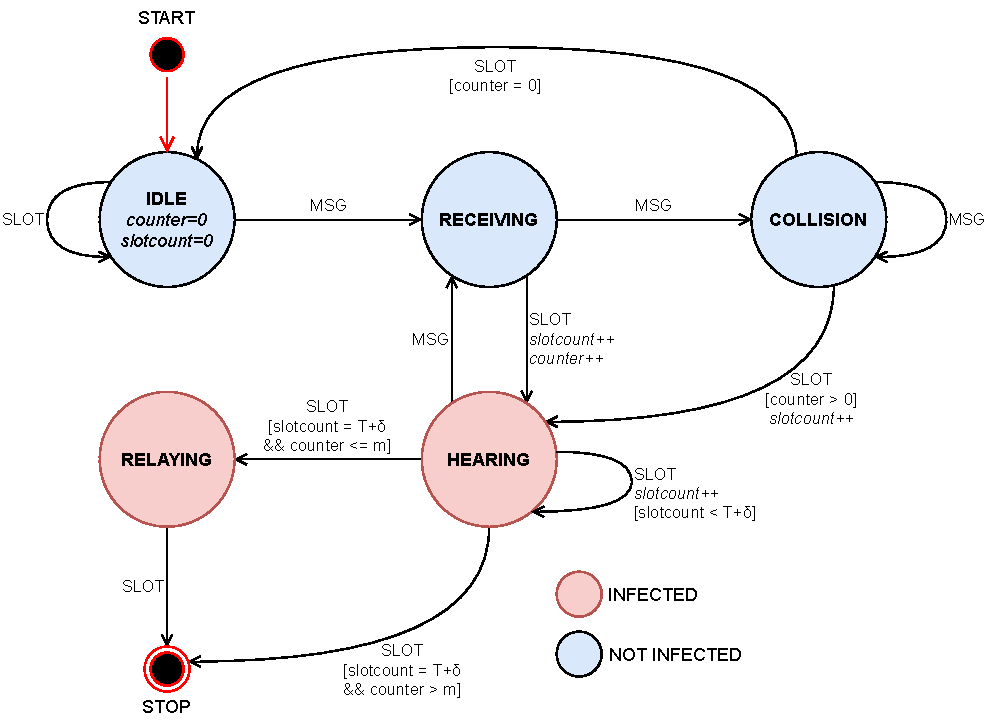
\includegraphics[width=\textwidth]{img/userfsm}
	\caption{FSM diagram of the \code{User} module}\label{fig:userfsm}
\end{figure}

We note that in our implementation of the \code{User} module, the transmission
of the message exchanged between users (\code{MSG}) does not really occupies an
entire slot (we have set its propagation delay equal to
\(\frac{\textrm{slotDuration}}{2}\)) in order to guarantee the order of events:
exchanged messages between users always come before self-messages used for
slotting, thus ensuring that the message is received in the current slot. In any
case, actual actions that the user should perform after a message is received
always take place in the next time slot.

The \code{Oracle} module is just a simple module that collects some ``global''
statistics and stops the simulation when no more activity is present in the
network \idest{No user is going to relay a message}. Users informs the oracle of
their actions via direct cross-module calls.

Note that also the oracle performs slotting, in order to properly be syncronized
with all other nodes when emitting statistic signals and to decrease the
\code{timeout} variable if no activity has been seen in the network during the
last slot. In order to ensure that the oracle always runs after all other nodes,
its self-messages used for slotting have been set to a lower scheduling
priority.
